\begin{adjustbox}{width=\textwidth}
	\begin{tikzpicture}[every node/.style={inner sep=0,outer sep=0}]
	
		\node [anchor=north east] (imgSpalten) at (-0.03\textwidth,0) {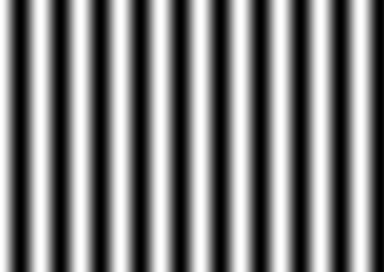
\includegraphics[frame,width=.47\textwidth]{02_grundlagenDerDeflektometrie/rekonstruktion/phasenKodierung/figures/sinusoidalesXMuster}};
		\node [below=0.2cm of imgSpalten, align = center] {Sinusoidales Muster zur Kodierung \\ der Spalten};
		\node [anchor=north west] (imgZeilen) at (0.03\textwidth,0) {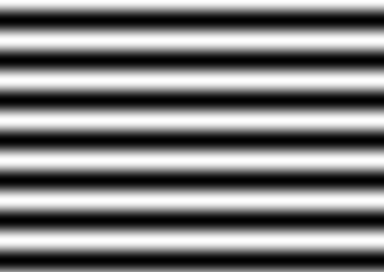
\includegraphics[frame,width=.47\textwidth]{02_grundlagenDerDeflektometrie/rekonstruktion/phasenKodierung/figures/sinusoidalesYMuster}};
		\node [below=0.2cm of imgZeilen, align = center] {Sinusoidales Muster zur Kodierung \\ der Zeilen};
		
	\end{tikzpicture}
\end{adjustbox}
\caption[Sinusoidale Streifenmuster]{Sinusoidale Streifenmuster zur Kodierung der Szene durch die Phasen $\left(\phi_x,\phi_y\right)$.}